\documentclass[a4paper,titlepage,11pt,twosides,floatssmall]{mwrep}
\usepackage[left=2.5cm,right=2.5cm,top=2.5cm,bottom=2.5cm]{geometry}
\usepackage[OT1]{fontenc}
\usepackage{polski}
\usepackage{amsmath}
\usepackage{amsfonts}
\usepackage{amssymb}
\usepackage{graphicx}
\usepackage{url}
\usepackage{tikz}
\usetikzlibrary{arrows,calc,decorations.markings,math,arrows.meta}
\usepackage{rotating}
\usepackage[percent]{overpic}
\usepackage[cp1250]{inputenc}
\usepackage{xcolor}
\usepackage{pgfplots}
\usetikzlibrary{pgfplots.groupplots}
\usepackage{listings}
\usepackage{matlab-prettifier}
\usepackage{enumitem,amssymb}
\definecolor{szary}{rgb}{0.95,0.95,0.95}
\usepackage{siunitx}
\sisetup{detect-weight,exponent-product=\cdot,output-decimal-marker={,},per-mode=symbol,binary-units=true,range-phrase={-},range-units=single}
\SendSettingsToPgf
%konfiguracje pakietu listings
\lstset{
	backgroundcolor=\color{szary},
	frame=single,
	breaklines=true,
}
\lstdefinestyle{customlatex}{
	basicstyle=\footnotesize\ttfamily,
	%basicstyle=\small\ttfamily,
}
\lstdefinestyle{customc}{
	breaklines=true,
	frame=tb,
	language=C,
	xleftmargin=0pt,
	showstringspaces=false,
	basicstyle=\small\ttfamily,
	keywordstyle=\bfseries\color{green!40!black},
	commentstyle=\itshape\color{purple!40!black},
	identifierstyle=\color{blue},
	stringstyle=\color{orange},
}
\lstdefinestyle{custommatlab}{
	captionpos=t,
	breaklines=true,
	frame=tb,
	xleftmargin=0pt,
	language=matlab,
	showstringspaces=false,
	%basicstyle=\footnotesize\ttfamily,
	basicstyle=\scriptsize\ttfamily,
	keywordstyle=\bfseries\color{green!40!black},
	commentstyle=\itshape\color{purple!40!black},
	identifierstyle=\color{blue},
	stringstyle=\color{orange},
}

%wymiar tekstu (bez �ywej paginy)
\textwidth 160mm \textheight 247mm

%ustawienia pakietu pgfplots
\pgfplotsset{
tick label style={font=\scriptsize},
label style={font=\small},
legend style={font=\small},
title style={font=\small}
}

\def\figurename{Rys.}
\def\tablename{Tab.}

%konfiguracja liczby p�ywaj�cych element�w
\setcounter{topnumber}{0}%2
\setcounter{bottomnumber}{3}%1
\setcounter{totalnumber}{5}%3
\renewcommand{\textfraction}{0.01}%0.2
\renewcommand{\topfraction}{0.95}%0.7
\renewcommand{\bottomfraction}{0.95}%0.3
\renewcommand{\floatpagefraction}{0.35}%0.5

\begin{document}
\frenchspacing
\pagestyle{uheadings}

%strona tytu�owa
\title{\bf Sprawozdanie z projektu i �wiczenia laboratoryjnego nr 2, zadanie nr 10\vskip 0.1cm}
\author{Karol Borowski, Szymon Koz�owski, Bartosz Kurpiewski}
\date{2019}

\makeatletter
\renewcommand{\maketitle}{\begin{titlepage}
\begin{center}{\LARGE {\bf
Wydzia� Elektroniki i Technik Informacyjnych}}\\
\vspace{0.4cm}
{\LARGE {\bf Politechnika Warszawska}}\\
\vspace{0.3cm}
\end{center}
\vspace{5cm}
\begin{center}
{\bf \LARGE Projektowanie uk�ad�w sterowania\\ (projekt grupowy) \vskip 0.1cm}
\end{center}
\vspace{1cm}
\begin{center}
{\bf \LARGE \@title}
\end{center}
\vspace{2cm}
\begin{center}
{\bf \Large \@author \par}
\end{center}
\vspace*{\stretch{6}}
\begin{center}
\bf{\large{Warszawa, \@date\vskip 0.1cm}}
\end{center}
\end{titlepage}
}
\makeatother

\maketitle

\tableofcontents
\chapter{Wst�p}
Tematem projektu i laboratorium pierwszego by�a implementacja, weryfikacja poprawno�ci dzia�ania i dob�r parametr�w algorytm�w regulacji jednowymiarowego procesu. W ramach projektu nale�a�o zasymulowa� i zbada� podany obiekt. Nast�pnie na podstawie uzyskanych wynik�w trzeba by�o zaimplementowa� regulator PID oraz DMC. Ostatnim krokiem by�o dostrojenie obu regulator�w, uwzgl�dniaj�c podane w projekcie ograniczenia.

W laboratorium pracowali�my na stanowisku grzej�co-ch�odz�cym. Celem pracy by�o wykorzystanie nabytych, podczas realizacji projektu, umiej�tno�ci do implementacji regulator�w na obiekcie rzeczywistym. Podczas �wicze� laboratoryjnych korzystali�my tylko z cz�ci element�w wykonawczych stanowiska: grza�ki \verb+G1+, wentylatora \verb+W1+ i czujnika temperatury \verb+T1+.
\chapter{Laboratorium}
\section{Zadanie 1}
Sprawdzaj�c komunikacj� ze stanowiskiem skorzystali�my z dw�ch funkcji zapewnionych przez prowadz�cego \verb+MinimalWorkingExample.m+ raz \verb+sendControlsToG1AndDisturbance.m+. Pierwsza z nich pozwala w prosty spos�b, konfiguruj�c port, na kt�rym odbywa si� komunikacja, zadawa� warto�ci sterowania na poszczeg�lne elementy wykonawcze stanowiska.
\begin{lstlisting}
        sendControls(1, 50);
\end{lstlisting}
Zadaj�c warto�� 0 i 50 na wentylator widzimy i s�yszymy czy komunikacja zachodzi.

Sterowanie grza�k� w tym zadaniu odbywa�o si� z u�yciem drugiej z wymienionych funkcji, aby zrealizowa� zadane w poleceniu zak��cenia. Funkcja \verb+sendControlsToG1AndDisturbance.m+ przyjmuje dwa argumenty: warto�� sterowania grza�k� \verb+G1+ i zak��cenia \verb+Z+.
\begin{lstlisting}
        sendControlsToG1AndDisturbance(35, Z);
\end{lstlisting}

Kolejnym krokiem by�o okre�lenie warto�ci temperatury w punkcie pracy: \verb+G1+ = 35, \verb+W1+ = 50, \verb+Z+ = 0. Dla takich nastaw temperatura wynosi�a ok. $32^{\mathrm{o}}{\mathrm{C}}$.
\section{Zadanie 2}
 Rozpoczynaj�c z punktu pracy - przy zerowym zak��ceniu - wyznaczyli�my trzy odpowiedzi skokowe toru zak��cenie-wyj�cie, wykonuj�c skoki sygna�u zak��caj�cego w chwili $k=0$ odpowiednio do warto�ci 10, 20 i 30. Wszystkie odpowiedzi przedstawione s� na rysunku $Rys. 2.1$.
\begin{figure}[tb]
\centering
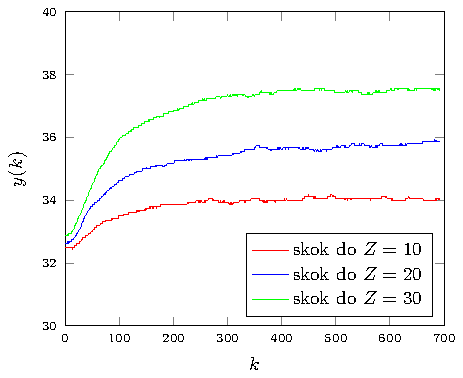
\includegraphics[scale=1]{rysunki/zad2plot}
\caption{Odpowiedzi skokowe toru zak��cenie-wyj�cie dla r�nych zmian sygna�u zak��caj�cego w chwili $k=0$}
\end{figure}
Wyznaczono charakterystyk� statyczn� ($Rys. 2.2.$). W�a�ciwo�ci statyczne obiektu mo�emy okre�li� jako (w przybli�eniu) liniowe.  Wzmocnienie statyczne dla tego toru wynosi w przybli�eniu $\num{0,15}$ - warto�� wsp�czynnika kierunkowego funkcji liniowej b�d�cej charakterystyk� statyczn�.
\begin{figure}[tb]
\centering
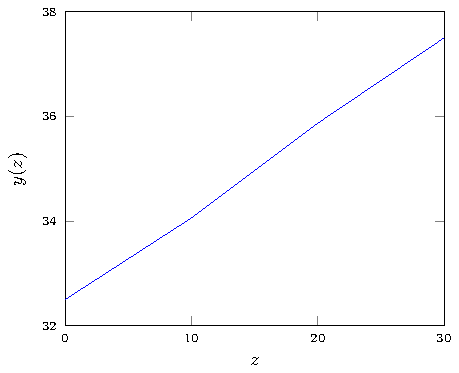
\includegraphics[scale=1]{rysunki/zad2char_st}
\caption{Charakterystyka statyczna - tor zak��cenie-wyj�cie}
\end{figure}
\section{Zadanie 3}
Przygotowujemy odpowied� skokow� toru wej�cie-wyj�cie tzn. zestaw liczb $s_1,s_2,...$ oraz odpowied� skokow� toru zak��cenie-wyj�cie tzn. zestaw liczb $s_1^z,s_2^z,...$ wykorzystywane w algorytmie DMC (odpowied� na skok jednostkowy w chwili $k = 0$). Dokonujemy poni�szych operacji na wektorach pobranych odpowiedzi skokowych obiektu.
\begin{equation}
s_i = \frac{y_i- Y_{\mathrm{pp}}}{\Delta U}, dla\ i=1,...
\end{equation}
\begin{equation}
s_i^z = \frac{y_i- Y_{\mathrm{pp}}}{\Delta Z}, dla\ i=1,...
\end{equation}
Wykorzystano odpowied� skokow� przy zmianie warto�ci $G1$ z 35 na 37 oraz odpowied� skokow� przy zmianie warto�ci $Z$ z 0 na 30. Odpowiedzi skokowe zaproksymowano u�ywaj�c cz�onu inercyjnego drugiego rz�du z op�nieniem. Zastosowano optymalizacj� � wyznaczenie takich warto�ci parametr�w $T_1$, $T_2$, $K$, $T_d$, aby warto�� funkcji celu (warto�� b��du dopasowania) by�a jak najmniejsza.
\begin{equation}
min\ E=\sum_{k=1}^{k_{\mathrm{max}}}(s(k)-y_{aproks}(k))^{2}
\end{equation}

Przyj�to nast�puj�ce ograniczenia parametr�w:
\begin{equation}
		0,001 \ll T_1 \ll 1000
\end{equation}
\begin{equation}
		0,001 \ll T_2 \ll 1000
\end{equation}
\begin{equation}
		-10 \ll K \ll 10
\end{equation}
\begin{equation}
		0 \ll T_d \ll 500
\end{equation}

Optymalizacji dokonano wykorzystuj�c funkcj� \verb+fmincon+, kt�ra znajduje minimum funkcji z uwzgl�dnieniem ogranicze�. Jedynymi ograniczeniami s� te, narzucone na argumenty wywo�ania funkcji celu, czyli na wy�ej okre�lone parametry. Kryteria zatrzymania algorytmu pozostawiono domy�lne. Podsumowuj�c, wynik algorytmu otrzymano przez zastosowanie polecenia: 
\begin{lstlisting}
[optim_params, E] = fmincon(fun, x0, [],[],[],[], lb, ub);
\end{lstlisting}
gdzie:
\begin{lstlisting}
optim_params � szukane parametry
E � b��d dopasowania
fun � funkcja zwracaj�ca warto�� b��du dopasowania
x0 � wektor parametr�w pocz�tkowych
lb � wektor dolnych ogranicze�
ub � wektor g�rnych ogranicze�
\end{lstlisting}
Wyznaczone parametry - tor sterowanie-wyj�cie:
$T_1 = \num{251,2387}, T_2 = \num{0,072366}, K = \num{0,48671}, T_{\mathrm{d}} = 6, E = \num{2,0984}$.
Wyznaczone parametry - tor zak��cenie-wyj�cie:
$T_1 = \num{89,0529}, T_2 = \num{2,1074}, K = \num{0,15435}, T_{\mathrm{d}} = 9, E = \num{0,0030778}$.

\begin{figure}[tb]
\centering
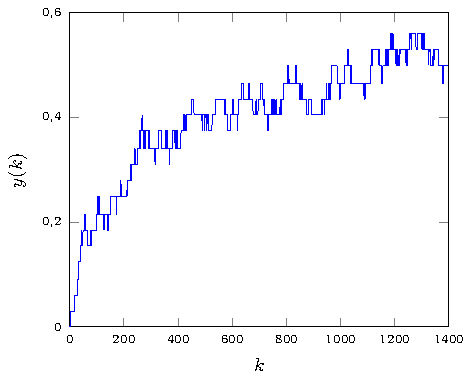
\includegraphics[scale=1]{rysunki/odp_sk_u}
\caption{Odpowied� skokowa toru wej�cie-wyj�cie wykorzystywana w algorytmie DMC}
\end{figure}
\begin{figure}[tb]
\centering
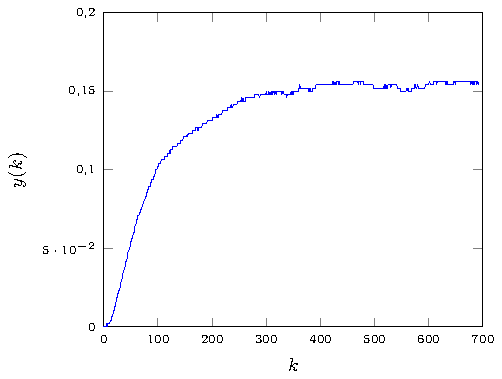
\includegraphics[scale=1]{rysunki/odp_sk_z}
\caption{Odpowied� skokowa toru zak��cenie-wyj�cie wykorzystywana w algorytmie DMC}
\end{figure}
\begin{figure}[tb]
\centering
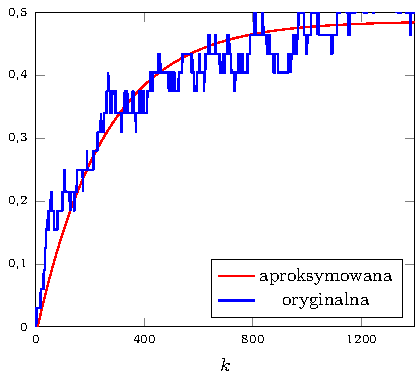
\includegraphics[scale=1]{rysunki/porownanie}
\caption{Por�wnanie oryginalnej odpowiedzi skokowej  toru wej�cie-wyj�cie z aproksymowan�}
\end{figure}
\begin{figure}[tb]
\centering
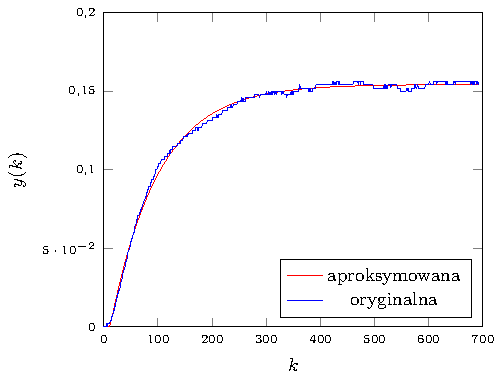
\includegraphics[scale=1]{rysunki/aprox_z}
\caption{Por�wnanie oryginalnej odpowiedzi skokowej toru zak��cenie-wyj�cie z aproksymowan�}
\end{figure}

\section{Zadanie 4}
Implementacja i opis programu znajduje si� w pliku \verb+DMC_lab.m+.

\subsection{Dob�r parametr�w algorytmu DMC przy zerowym zak��ceniu}
Eksperyment rozpocz�to od nast�puj�cych parametr�w: $N = N_{\mathrm{u}} = D = 1395$, $\lambda=1$ ($Rys.\ 2.7$). $D$ przyj�to jako d�ugo�� wektora pobranej odpowiedzi skokowej. Warto�ci horyzont�w zmniejszono do 80 ($Rys.\ 2.8$). Warto�� wska�nika jako�ci uda�o si� minimalnie zmniejszy�, jednak dalej jest ona zbyt du�a. Uk�ad dzia�a wolno, wyst�puje niezerowe przeregulowanie. Nast�pnie eksperyment polega� na stopniowym zmniejszaniu horyzontu sterowania ($Rys.\ 2.9$). Warto�� wska�nika jako�ci zmniejszy�a si� o ok. 10\%. Przy dalszym zmniejszaniu warto�ci horyzontu sterowania suma kwadrat�w uchyb�w ro�nie ($Rys.\ 2.10$).

Najwi�ksz� zmian� przynios�a zmiana parametru $\lambda$ � parametru kar za przyrosty sterowania. Jego zwi�kszenie powoduje jeszcze wolniejsz� prac� uk�adu regulacji ($Rys.\ 2.11$). Natomiast zmniejszenie znacznie przyspiesza reakcj� uk�adu na zmian� warto�ci zadanej ($Rys.\ 2.12$). Dalsze zmniejszenie parametru lambda przynosi jeszcze bardziej gwa�towne zmiany sterowania oraz zwi�kszenie oscylacji temperatury ($Rys.\ 2.13$). Warto�� wska�nika jako�ci jest mniejsza. Jednak przy wyborze parametru $\lambda$ istotne s� zmiany sygna�u sterowania, kt�re mog� by� niebezpieczne dla obiektu, gdy s� zbyt gwa�towne. Dlatego zdecydowali�my si� na warto�� parametru $\lambda=1$. Eksperyment zako�czono wybieraj�c nast�puj�ce parametry algorytmu: $N = 80, N_{\mathrm{u}} = 25, \lambda = 1$.

%1
\begin{figure}[H]
	\centering
	\begin{tikzpicture}
	\begin{axis}[
	width=5.1in,
	height=1.4in,
	xmin=0,xmax=295,ymin=30,ymax=65,
	xlabel={$k$},
	ylabel={$U(k)$},
	legend pos=south east,
	y tick label style={/pgf/number format/1000 sep=},
	]
	\addplot[const plot,blue] file {rysunki/data/u(N=D,Nu=D,l=1).csv};
	\end{axis}
	\end{tikzpicture}
	\begin{tikzpicture}
	\begin{axis}[
	width=5.1in,
	height=1.4in,
	xmin=0,xmax=295,ymin=34,ymax=42,
	xlabel={$k$},
	ylabel={$Y(k)$,$Y^{\mathrm{zad}}(k)$},
	legend pos=south east,
	y tick label style={/pgf/number format/1000 sep=},
	]
	\addplot[const plot,blue] file {rysunki/data/y(N=D,Nu=D,l=1).csv};
	\addplot[const plot,red] file {rysunki/data/yzad.csv};
	\legend{$Y(k)$,$Y^{\mathrm{zad}}(k)$}
	\end{axis}
	\end{tikzpicture}
	\caption{Odpowied� uk�adu przy sterowaniu algorytmem DMC z parametrami
	\newline$N = N_{\mathrm{u}} = D = 1395, \lambda = 1, E = 454$}
\end{figure}

%2
\begin{figure}[H]
	\centering
	\begin{tikzpicture}
	\begin{axis}[
	width=5.1in,
	height=1.4in,
	xmin=0,xmax=295,ymin=30,ymax=65,
	xlabel={$k$},
	ylabel={$U(k)$},
	legend pos=south east,
	y tick label style={/pgf/number format/1000 sep=},
	]
	\addplot[const plot,blue] file {rysunki/data/u(N=Nu=80,l=1).csv};
	\end{axis}
	\end{tikzpicture}
	\begin{tikzpicture}
	\begin{axis}[
	width=5.1in,
	height=1.4in,
	xmin=0,xmax=295,ymin=34,ymax=42,
	xlabel={$k$},
	ylabel={$Y(k)$,$Y^{\mathrm{zad}}(k)$},
	legend pos=south east,
	y tick label style={/pgf/number format/1000 sep=},
	]
	\addplot[const plot,blue] file {rysunki/data/y(N=Nu=80,l=1).csv};
	\addplot[const plot,red] file {rysunki/data/yzad.csv};
	\legend{$Y(k)$,$Y^{\mathrm{zad}}(k)$}
	\end{axis}
	\end{tikzpicture}
	\caption{Odpowied� uk�adu przy sterowaniu algorytmem DMC z parametrami
	\newline$N = N_{\mathrm{u}} = 80, \lambda = 1, E = 440$}
\end{figure}

%3
\begin{figure}[H]
	\centering
	\begin{tikzpicture}
	\begin{axis}[
	width=5.1in,
	height=1.4in,
	xmin=0,xmax=295,ymin=30,ymax=65,
	xlabel={$k$},
	ylabel={$U(k)$},
	legend pos=south east,
	y tick label style={/pgf/number format/1000 sep=},
	]
	\addplot[const plot,blue] file {rysunki/data/u(N=80,Nu=25,l=1).csv};
	\end{axis}
	\end{tikzpicture}
	\begin{tikzpicture}
	\begin{axis}[
	width=5.1in,
	height=1.4in,
	xmin=0,xmax=295,ymin=34,ymax=42,
	xlabel={$k$},
	ylabel={$Y(k)$,$Y^{\mathrm{zad}}(k)$},
	legend pos=south east,
	y tick label style={/pgf/number format/1000 sep=},
	]
	\addplot[const plot,blue] file {rysunki/data/y(N=80,Nu=25,l=1).csv};
	\addplot[const plot,red] file {rysunki/data/yzad.csv};
	\legend{$Y(k)$,$Y^{\mathrm{zad}}(k)$}
	\end{axis}
	\end{tikzpicture}
	\caption{Odpowied� uk�adu przy sterowaniu algorytmem DMC z parametrami
	\newline$N = 80, N_{\mathrm{u}} = 25, \lambda = 1, E = 405$}
\end{figure}

%4
\begin{figure}[H]
	\centering
	\begin{tikzpicture}
	\begin{axis}[
	width=5.1in,
	height=1.4in,
	xmin=0,xmax=295,ymin=30,ymax=65,
	xlabel={$k$},
	ylabel={$U(k)$},
	legend pos=south east,
	y tick label style={/pgf/number format/1000 sep=},
	]
	\addplot[const plot,blue] file {rysunki/data/u(N=80,Nu=10,l=1).csv};
	\end{axis}
	\end{tikzpicture}
	\begin{tikzpicture}
	\begin{axis}[
	width=5.1in,
	height=1.4in,
	xmin=0,xmax=295,ymin=34,ymax=42,
	xlabel={$k$},
	ylabel={$Y(k)$,$Y^{\mathrm{zad}}(k)$},
	legend pos=south east,
	y tick label style={/pgf/number format/1000 sep=},
	]
	\addplot[const plot,blue] file {rysunki/data/y(N=80,Nu=10,l=1).csv};
	\addplot[const plot,red] file {rysunki/data/yzad.csv};
	\legend{$Y(k)$,$Y^{\mathrm{zad}}(k)$}
	\end{axis}
	\end{tikzpicture}
	\caption{Odpowied� uk�adu przy sterowaniu algorytmem DMC z parametrami
	\newline$N = 80, N_{\mathrm{u}} = 10, \lambda = 1, E = 454$}
\end{figure}

%5
\begin{figure}[H]
	\centering
	\begin{tikzpicture}
	\begin{axis}[
	width=5.1in,
	height=1.4in,
	xmin=0,xmax=295,ymin=30,ymax=60,
	xlabel={$k$},
	ylabel={$U(k)$},
	legend pos=south east,
	y tick label style={/pgf/number format/1000 sep=},
	]
	\addplot[const plot,blue] file {rysunki/data/u(N=80,Nu=25,l=10).csv};
	\end{axis}
	\end{tikzpicture}
	\begin{tikzpicture}
	\begin{axis}[
	width=5.1in,
	height=1.4in,
	xmin=0,xmax=295,ymin=34,ymax=42,
	xlabel={$k$},
	ylabel={$Y(k)$,$Y^{\mathrm{zad}}(k)$},
	legend pos=south east,
	y tick label style={/pgf/number format/1000 sep=},
	]
	\addplot[const plot,blue] file {rysunki/data/y(N=80,Nu=25,l=10).csv};
	\addplot[const plot,red] file {rysunki/data/yzad.csv};
	\legend{$Y(k)$,$Y^{\mathrm{zad}}(k)$}
	\end{axis}
	\end{tikzpicture}
	\caption{Odpowied� uk�adu przy sterowaniu algorytmem DMC z parametrami
	\newline$N = 80, N_{\mathrm{u}} = 25, \lambda = 10, E = 543$}
\end{figure}

%6
\begin{figure}[H]
	\centering
	\begin{tikzpicture}
	\begin{axis}[
	width=5.1in,
	height=1.4in,
	xmin=0,xmax=295,ymin=30,ymax=80,
	xlabel={$k$},
	ylabel={$U(k)$},
	legend pos=south east,
	y tick label style={/pgf/number format/1000 sep=},
	]
	\addplot[const plot,blue] file {rysunki/data/u(N=80,Nu=25,l=0.1).csv};
	\end{axis}
	\end{tikzpicture}
	\begin{tikzpicture}
	\begin{axis}[
	width=5.1in,
	height=1.4in,
	xmin=0,xmax=295,ymin=34,ymax=42,
	xlabel={$k$},
	ylabel={$Y(k)$,$Y^{\mathrm{zad}}(k)$},
	legend pos=south east,
	y tick label style={/pgf/number format/1000 sep=},
	]
	\addplot[const plot,blue] file {rysunki/data/y(N=80,Nu=25,l=0.1).csv};
	\addplot[const plot,red] file {rysunki/data/yzad.csv};
	\legend{$Y(k)$,$Y^{\mathrm{zad}}(k)$}
	\end{axis}
	\end{tikzpicture}
	\caption{Odpowied� uk�adu przy sterowaniu algorytmem DMC z parametrami
	\newline$N = 80, N_{\mathrm{u}} = 25, \lambda = \num{0.1}, E = 327$}
\end{figure}

%7
\begin{figure}[H]
	\centering
	\begin{tikzpicture}
	\begin{axis}[
	width=5.1in,
	height=1.4in,
	xmin=0,xmax=295,ymin=10,ymax=100,
	xlabel={$k$},
	ylabel={$U(k)$},
	legend pos=south east,
	y tick label style={/pgf/number format/1000 sep=},
	]
	\addplot[const plot,blue] file {rysunki/data/u(N=80,Nu=25,l=0.01).csv};
	\end{axis}
	\end{tikzpicture}
	\begin{tikzpicture}
	\begin{axis}[
	width=5.1in,
	height=1.4in,
	xmin=0,xmax=295,ymin=34,ymax=42,
	xlabel={$k$},
	ylabel={$Y(k)$,$Y^{\mathrm{zad}}(k)$},
	legend pos=south east,
	y tick label style={/pgf/number format/1000 sep=},
	]
	\addplot[const plot,blue] file {rysunki/data/y(N=80,Nu=25,l=0.01).csv};
	\addplot[const plot,red] file {rysunki/data/yzad.csv};
	\legend{$Y(k)$,$Y^{\mathrm{zad}}(k)$}
	\end{axis}
	\end{tikzpicture}
	\caption{Odpowied� uk�adu przy sterowaniu algorytmem DMC z parametrami
	\newline$N = 80, N_{\mathrm{u}} = 25, \lambda = \num{0.01}, E = 290$}
\end{figure}
\section{Zadanie 5}
Parametr $D^{\mathrm{z}}$ jest warto�ci� okre�laj�c� liczb� krok�w zak��ce�, kt�re uwzgl�dniamy. Dobrano go jako liczb� pr�bek, po kt�rej odpowied� skokowa toru zak��cenie-wyj�cie wykorzystywana w algorytmie DMC stabilizuje si�. $D^{\mathrm{z}}=400$.

Nast�pnie wykonano eksperymenty, w kt�rych po zmianie warto�ci zadanej i ustabilizowaniu si� temperatury obiektu nast�puj� zmiany sygna��w zak��ce�.
Zebrano wyniki dla trzech r�nych trajektorii zak��ce� wykorzystuj�c odpowiednio algorytm bez pomiaru zak��ce� i z pomiarem zak��ce�.

%1
\begin{figure}[H]
	\centering
	\begin{tikzpicture}
	\begin{axis}[
	width=5.1in,
	height=1.5in,
	xmin=0,xmax=247,ymin=30,ymax=70,
	xlabel={$k$},
	ylabel={$U(k)$},
	legend pos=south east,
	y tick label style={/pgf/number format/1000 sep=},
	]
	\addplot[const plot,blue] file {rysunki/data/u(bez0_30).csv};
	\end{axis}
	\end{tikzpicture}
	\begin{tikzpicture}
	\begin{axis}[
	width=5.1in,
	height=1.1in,
	xmin=0,xmax=247,ymin=0,ymax=30,
	xlabel={$k$},
	ylabel={$Z(k)$},
	legend pos=south east,
	y tick label style={/pgf/number format/1000 sep=},
	]
	\addplot[const plot,blue] file {rysunki/data/z0_30.csv};
	\end{axis}
	\end{tikzpicture}
	\begin{tikzpicture}
	\begin{axis}[
	width=5.1in,
	height=1.75in,
	xmin=0,xmax=247,ymin=33,ymax=40,
	xlabel={$k$},
	ylabel={$Y(k)$, $Y^{\mathrm{zad}}(k)$},
	legend pos=south east,
	y tick label style={/pgf/number format/1000 sep=},
	]
	\addplot[const plot,blue] file {rysunki/data/y(bez0_30).csv};
	\addplot[const plot,red] file {rysunki/data/yzad(0_30).csv};
	\legend{$Y(k)$, $Y^{\mathrm{zad}}(k)$}
	\end{axis}
	\end{tikzpicture}
	\caption{Regulacja obiektu algorytmem DMC bez uwzgl�dnienia pomiaru zak��ce�}
\end{figure}

%2
\begin{figure}[H]
	\centering
	\begin{tikzpicture}
	\begin{axis}[
	width=5.1in,
	height=1.5in,
	xmin=0,xmax=247,ymin=30,ymax=70,
	xlabel={$k$},
	ylabel={$U(k)$},
	legend pos=south east,
	y tick label style={/pgf/number format/1000 sep=},
	]
	\addplot[const plot,blue] file {rysunki/data/u(uwz0_30).csv};
	\end{axis}
	\end{tikzpicture}
	\begin{tikzpicture}
	\begin{axis}[
	width=5.1in,
	height=1.1in,
	xmin=0,xmax=247,ymin=0,ymax=30,
	xlabel={$k$},
	ylabel={$Z(k)$},
	legend pos=south east,
	y tick label style={/pgf/number format/1000 sep=},
	]
	\addplot[const plot,blue] file {rysunki/data/z0_30.csv};
	\end{axis}
	\end{tikzpicture}
	\begin{tikzpicture}
	\begin{axis}[
	width=5.1in,
	height=1.75in,
	xmin=0,xmax=247,ymin=33,ymax=40,
	xlabel={$k$},
	ylabel={$Y(k)$, $Y^{\mathrm{zad}}(k)$},
	legend pos=south east,
	y tick label style={/pgf/number format/1000 sep=},
	]
	\addplot[const plot,blue] file {rysunki/data/y(uwz0_30).csv};
	\addplot[const plot,red] file {rysunki/data/yzad(0_30).csv};
	\legend{$Y(k)$, $Y^{\mathrm{zad}}(k)$}
	\end{axis}
	\end{tikzpicture}
	\caption{Regulacja obiektu algorytmem DMC z uwzgl�dnieniem pomiaru zak��ce�}
\end{figure}

%3
\begin{figure}[H]
	\centering
	\begin{tikzpicture}
	\begin{axis}[
	width=5.1in,
	height=1.5in,
	xmin=0,xmax=497,ymin=0,ymax=70,
	xlabel={$k$},
	ylabel={$U(k)$},
	legend pos=south east,
	y tick label style={/pgf/number format/1000 sep=},
	]
	\addplot[const plot,blue] file {rysunki/data/u(bez0_30_70).csv};
	\end{axis}
	\end{tikzpicture}
	\begin{tikzpicture}
	\begin{axis}[
	width=5.1in,
	height=1.1in,
	xmin=0,xmax=497,ymin=0,ymax=70,
	xlabel={$k$},
	ylabel={$Z(k)$},
	legend pos=south east,
	y tick label style={/pgf/number format/1000 sep=},
	]
	\addplot[const plot,blue] file {rysunki/data/z(bez0_30_70).csv};
	\end{axis}
	\end{tikzpicture}
	\begin{tikzpicture}
	\begin{axis}[
	width=5.1in,
	height=1.75in,
	xmin=0,xmax=497,ymin=33,ymax=42,
	xlabel={$k$},
	ylabel={$Y(k)$, $Y^{\mathrm{zad}}(k)$},
	legend pos=south east,
	y tick label style={/pgf/number format/1000 sep=},
	]
	\addplot[const plot,blue] file {rysunki/data/y(bez0_30_70).csv};
	\addplot[const plot,red] file {rysunki/data/yzad(0_30_70).csv};
	\legend{$Y(k)$, $Y^{\mathrm{zad}}(k)$}
	\end{axis}
	\end{tikzpicture}
	\caption{Regulacja obiektu algorytmem DMC bez uwzgl�dnienia pomiaru zak��ce�}
\end{figure}

%4
\begin{figure}[H]
	\centering
	\begin{tikzpicture}
	\begin{axis}[
	width=5.1in,
	height=1.5in,
	xmin=0,xmax=495,ymin=0,ymax=70,
	xlabel={$k$},
	ylabel={$U(k)$},
	legend pos=south east,
	y tick label style={/pgf/number format/1000 sep=},
	]
	\addplot[const plot,blue] file {rysunki/data/u(uwz0_30_70).csv};
	\end{axis}
	\end{tikzpicture}
	\begin{tikzpicture}
	\begin{axis}[
	width=5.1in,
	height=1.1in,
	xmin=0,xmax=495,ymin=0,ymax=70,
	xlabel={$k$},
	ylabel={$Z(k)$},
	legend pos=south east,
	y tick label style={/pgf/number format/1000 sep=},
	]
	\addplot[const plot,blue] file {rysunki/data/z(uwz0_30_70).csv};
	\end{axis}
	\end{tikzpicture}
	\begin{tikzpicture}
	\begin{axis}[
	width=5.1in,
	height=1.75in,
	xmin=0,xmax=495,ymin=33,ymax=42,
	xlabel={$k$},
	ylabel={$Y(k)$, $Y^{\mathrm{zad}}(k)$},
	legend pos=south east,
	y tick label style={/pgf/number format/1000 sep=},
	]
	\addplot[const plot,blue] file {rysunki/data/y(uwz0_30_70).csv};
	\addplot[const plot,red] file {rysunki/data/yzad(0_30_70).csv};
	\legend{$Y(k)$, $Y^{\mathrm{zad}}(k)$}
	\end{axis}
	\end{tikzpicture}
	\caption{Regulacja obiektu algorytmem DMC z uwzgl�dnieniem pomiaru zak��ce�}
\end{figure}

%5
\begin{figure}[H]
	\centering
	\begin{tikzpicture}
	\begin{axis}[
	width=5.1in,
	height=1.5in,
	xmin=0,xmax=594,ymin=0,ymax=70,
	xlabel={$k$},
	ylabel={$U(k)$},
	legend pos=south east,
	y tick label style={/pgf/number format/1000 sep=},
	]
	\addplot[const plot,blue] file {rysunki/data/u(bez0_60_20).csv};
	\end{axis}
	\end{tikzpicture}
	\begin{tikzpicture}
	\begin{axis}[
	width=5.1in,
	height=1.1in,
	xmin=0,xmax=594,ymin=0,ymax=60,
	xlabel={$k$},
	ylabel={$Z(k)$},
	legend pos=south east,
	y tick label style={/pgf/number format/1000 sep=},
	]
	\addplot[const plot,blue] file {rysunki/data/z(bez0_60_20).csv};
	\end{axis}
	\end{tikzpicture}
	\begin{tikzpicture}
	\begin{axis}[
	width=5.1in,
	height=1.75in,
	xmin=0,xmax=594,ymin=33,ymax=42,
	xlabel={$k$},
	ylabel={$Y(k)$, $Y^{\mathrm{zad}}(k)$},
	legend pos=south east,
	y tick label style={/pgf/number format/1000 sep=},
	]
	\addplot[const plot,blue] file {rysunki/data/y(bez0_60_20).csv};
	\addplot[const plot,red] file {rysunki/data/yzad(0_60_20).csv};
	\legend{$Y(k)$, $Y^{\mathrm{zad}}(k)$}
	\end{axis}
	\end{tikzpicture}
	\caption{Regulacja obiektu algorytmem DMC bez uwzgl�dnienia pomiaru zak��ce�}
\end{figure}

%6
\begin{figure}[H]
	\centering
	\begin{tikzpicture}
	\begin{axis}[
	width=5.1in,
	height=1.5in,
	xmin=0,xmax=595,ymin=0,ymax=70,
	xlabel={$k$},
	ylabel={$U(k)$},
	legend pos=south east,
	y tick label style={/pgf/number format/1000 sep=},
	]
	\addplot[const plot,blue] file {rysunki/data/u(uwz0_60_20).csv};
	\end{axis}
	\end{tikzpicture}
	\begin{tikzpicture}
	\begin{axis}[
	width=5.1in,
	height=1.1in,
	xmin=0,xmax=595,ymin=0,ymax=70,
	xlabel={$k$},
	ylabel={$Z(k)$},
	legend pos=south east,
	y tick label style={/pgf/number format/1000 sep=},
	]
	\addplot[const plot,blue] file {rysunki/data/z(uwz0_60_20).csv};
	\end{axis}
	\end{tikzpicture}
	\begin{tikzpicture}
	\begin{axis}[
	width=5.1in,
	height=1.75in,
	xmin=0,xmax=595,ymin=33,ymax=42,
	xlabel={$k$},
	ylabel={$Y(k)$, $Y^{\mathrm{zad}}(k)$},
	legend pos=south east,
	y tick label style={/pgf/number format/1000 sep=},
	]
	\addplot[const plot,blue] file {rysunki/data/y(uwz0_60_20).csv};
	\addplot[const plot,red] file {rysunki/data/yzad(0_60_20).csv};
	\legend{$Y(k)$, $Y^{\mathrm{zad}}(k)$}
	\end{axis}
	\end{tikzpicture}
	\caption{Regulacja obiektu algorytmem DMC z uwzgl�dnieniem pomiaru zak��ce�}
\end{figure}

Uwzgl�dnienie zak��ce� poprawi�o dzia�anie uk�adu regulacji. Wida� to szczeg�lnie przy jednokrotnym skoku zak��cenia ($Rys.\ 2.15$). Uk�ad szybko reaguje na zmian� zak��cenia, obni�aj�c warto�� sygna�u sterowania. Pozwala to na utrzymanie temperatury zadanej mimo sta�ych zak��ce�. Natomiast przy braku uwzgl�dnienia zak��ce� ($Rys.\ 2.14$) pojawia si� uchyb - temperatura odbiega od warto�ci zadanej po wyst�pieniu zak��ce�.
Dla kolejnych trajektorii zak��ce� - dwukrotnego skoku, uk�ad dzia�a gorzej. Kiedy jeszcze pierwsz� zmian� zak��ce� udaje si� w miar� skompensowa� ($Rys.\ 2.17$, $Rys.\ 2.19$), tak rozpoczynaj�c z innego punktu pracy, zmiana zak��ce� prowadzi do destabilizacji uk�adu. Oczywi�cie, algorytm bez uwzgl�dnienia pomiaru zak��ce� tak�e nie jest w stanie utrzyma� warto�ci zadanej. Jednak jako�� regulacji jest jeszcze mniejsza.

\appendix

\end{document}

